% Copyright 2021 Néstor Nápoles López

% This is \refsubsec{automaticpitchspelling}, which
% introduces the automatic pitch spelling.

A pitch-spelling model is an algorithm that predicts the
original spelling that a note had in a musical score when
only the pitch-class, octave, and duration of the note are
provided as inputs to the model.\footnote{Some researchers
have also found helpful to know the voice (\emph{stream}, in
psychoacoustics) in which the note is sounding. However,
this information departs from what can be reliably obtained
from real-world digital music files. Therefore, a real-world
algorithm should work regardless of whether it knows what
voice played the note.}

% To understand the problems that derive from
% pitch-spelling, the following example could be considered.
% If during a musical performance, a pianist presses the key
% corresponding to the pitch class number 8 in the piano
% keyboard (shown in Figure  \ref{fig:Q7_1}), how can we
% know if the note played by the performer was an A$\flat$
% or a G$\sharp$?\footnote{Assume an equal-tempered setting,
% with no special considerations regarding how the piano
% might be tuned. That is, the distinction between the
% A$\flat$ and G$\sharp$ notes that we are looking for is of
% a semantic nature.}

% % \begin{figure}[h] \centering %
% 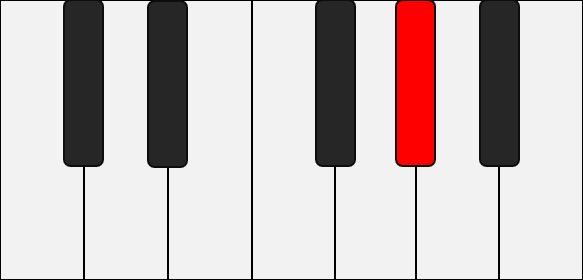
\includegraphics[width=0.6\textwidth]{figures/Q7_1.png} %
% \caption{A note playing in a keyboard. It could be %
% either G$\sharp$ or A$\flat$.} \label{fig:Q7_1} %
% \end{figure}

% This example problem may seem ingenuous at first, however,
% the spelling of a note could \emph{carry} much more
% information about the tonal context of the music that one
% might expect. Similarly, the reverse problem (spelling the
% note) may \emph{require} much more information about the
% tonal context of the music that one might expect. This
% double relationship between the acquired and delivered
% musical knowledge in the spelling of a note is what makes
% it an interesting computational problem, as it provides a
% framework for assessing quantitatively the extent to which
% a computational model understands the musical semantics.
% Furthermore, finding the spelling of a note has the
% additional advantage of being highly unambiguous as an
% evaluation metric compared to other analytical tasks like
% finding the musical key \parencite{gebhardt2018confidence}
% or labeling the chords in a piece
% \parencite{ni2013understanding}.

% In order to better contextualize what is the information
% contained in the spelling of a pitch, let us extend the
% previous thought exercise a bit further.

% A first impulse that someone might have for guessing
% whether the note is A$\flat$ or G$\sharp$ could be to know
% the musical key of the piece during which the piano key
% was played. Such information can be obtained from a
% key-finding model and there are many approaches that could
% provide it with a reasonable degree of accuracy.
% Nevertheless, our pitch-spelling model now requires
% information about the key in order to make its
% predictions.

% It could be assumed that the model will receive such
% predictions, and that they are reliable. A key-finding
% model could then inform us that the piece was in \emph{A
% minor}. ``Is it a piece in A minor?'' Then the note is
% probably a G$\sharp$.

% % \begin{figure}[h] \centering %
% 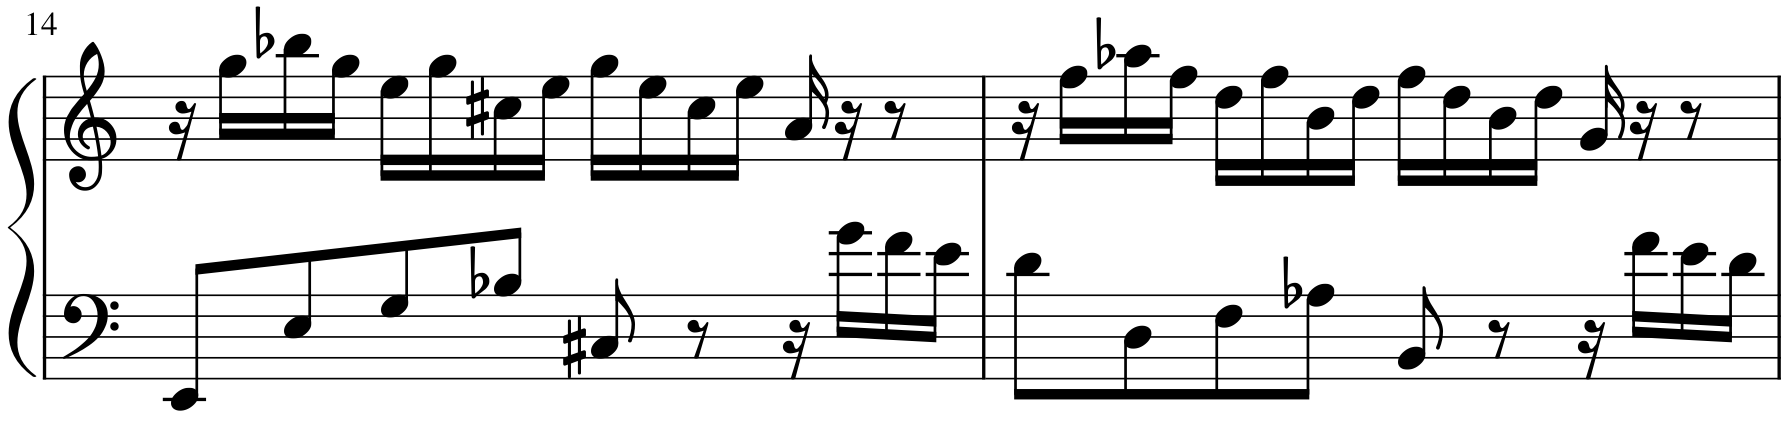
\includegraphics[width=0.8\textwidth]{figures/Q7_2.png} %
% \caption{J. S. Bach's BWV 784, mm. 14-15. The piece is %
% in A minor, however, during measure 15, the pitch %
% class number 8 is spelled as an A$\flat$.} %
% \label{fig:Q7_2} \end{figure}

% Figure \ref{fig:Q7_2} shows an adversarial example where
% the pitch class number 8 is spelled as A$\flat$ in a piece
% that is originally in \emph{A minor}. A person
% familiarized with Western tonal music could guess that
% similar examples as the one shown in Figure \ref{fig:Q7_2}
% will occur whenever the music is modulating or tonicizing
% a different key.

% Assuming that the awareness of modulations and
% tonicizations throughout the piece (which we generally
% refer to as \emph{local keys}) will mitigate our problems
% when predicting the spelling of a note, seems to be a
% reasonable guess. Instead of requiring to know the
% \emph{global key} of the piece, now, our model requires to
% know the \emph{local keys} throughout the piece. Notice,
% however, that there are much less models available that
% provide such information, and that there is no sufficient
% amount of research assessing whether they are accurate or
% not, mostly because the concepts of modulation and
% tonicization are problematic and ambiguous themselves (see
% Question \ref{chap:chap6} for a further discussion on
% modulation and tonicization).

% To complicate the matter a bit further, there are other
% circumstances that affect the spelling of a note, such as
% the use of non-chord tones or the harmonic context. One
% example of the implications of non-chord tones is, as
% shown in Figure \ref{fig:Q7_3}, the spelling of a
% chromatic neighbouring note, which should probably have a
% different note name than the \emph{real} note.

% % \begin{figure}[h] \centering %
% 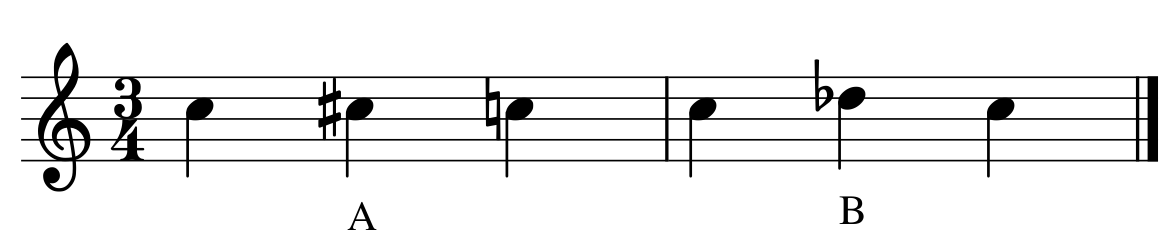
\includegraphics[width=0.8\textwidth]{figures/Q7_3.png} %
% \caption{Two notations (A and B) of a chromatic %
% neighbouring note. Regardless of the harmonic and key %
% context, the second note should probably be spelled as %
% in version B.} \label{fig:Q7_3} \end{figure}

% One example of a complicated harmonic context is the
% presence of a German augmented sixth, for which Teodoru
% and Raphael write \parencite{teodoru2007pitch}:
% \emph{Other situations require a deeper notion of the
% harmonic state than provided by the local key, as in the
% German augmented sixth chord, which seems nearly
% impossible to spell correctly without recognizing it as
% such.}

% Overall, designing a pitch-spelling algorithm poses
% important challenges in different musical fronts, but it
% also provides researchers with the opportunity of putting
% in practice different analytical models (e.g., local key,
% chord labeling, and non-chord detection) for solving a
% common task. Furthermore, unlike many of those models
% which suffer from highly ambiguous evaluations, pitch
% spelling presents a simple way of assessing whether our
% computational models understand the musical context or
% not. That is, the note is either G$\sharp$ or A$\flat$,
% and there is only one right answer.

% In the following section, a survey is provided with
% different pitch-spelling algorithms that have been
% developed throughout the years.

\guide{A brief survey of pitch-spelling algorithms}

Compared to other tasks of Music Information Retrieval
(MIR), there have not been as many attempts to solve the
problem of pitch spelling. Nevertheless, it is likely that
there are other solutions to the problem, in commercial
applications, which are not described in the literature and
in this survey. This is due to the fact that pitch-spelling
is a highly relevant problem for commercial software that
deals with the conversion of MIDI files into music scores,
for example, most music notation editors.

The reason why I consider pitch spelling to be a relevant problem for Roman numeral analysis is because recent models have benefitted from spelling information \parencite{micchi2020not}. This approach works for MusicXML inputs and similar symbolic representations, but not for MIDI inputs, which arguably account for the vast majority of the existing digital symbolic music files today. Pitch spelling in parallel (or as a preprocessing step) will be necessary for Roman numeral analysis then. This is also true for implementing Roman numeral analysis models in the audio domain.
